\documentclass[a4paper,12pt]{article}
\usepackage{mathtools,amsfonts,amssymb,amsmath, bm,commath,multicol}
\usepackage{algorithmicx, tkz-graph, algorithm, fancyhdr, pgfplots}
\usepackage{fancyvrb}

\usepackage[noend]{algpseudocode}

\DefineVerbatimEnvironment{juliaout}{Verbatim}{}
\DefineVerbatimEnvironment{juliacode}{Verbatim}{fontshape=sl, fontsize=\tiny}
\DefineVerbatimEnvironment{juliaterm}{Verbatim}{}


\begin{document}

\section*{5}
This question is most easily explained by overlaying the PDF's of the two classes:

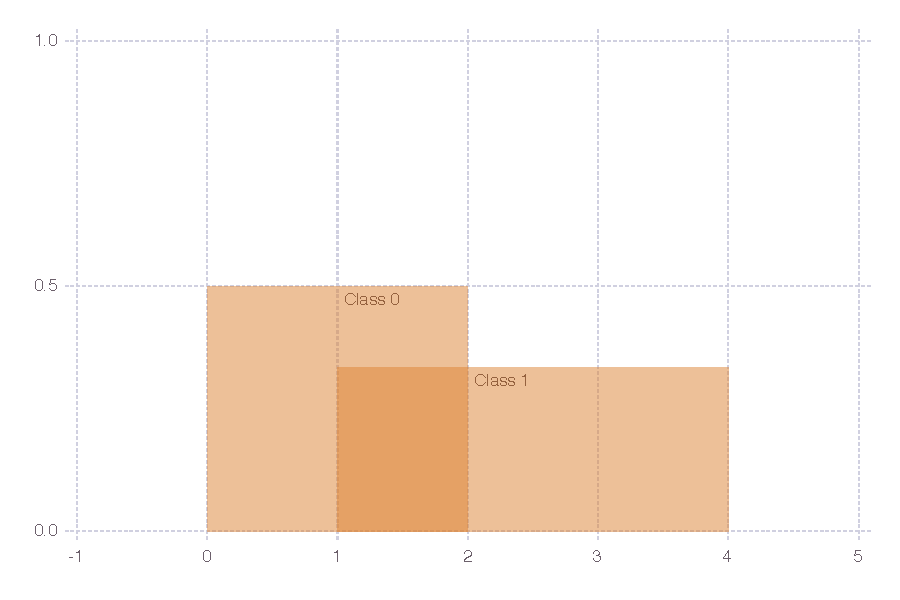
\includegraphics[width=\linewidth]{figures/weave-test_1_1.pdf}

The bayes classifier is very simple, from 0-2, pick 0, while from 2-4, you pick 1. The Bayes risk is simply the overlapping area in the graph of the two PDF's. When values are between 1-2, there is a risk of 2/5. This is obtained by summing all the possibilities to obtain our marginilizing constant, and then taking the density of class 1 over the area (1/3):

\begin{align*}
\frac{\frac{1}{3}}{\frac{1}{3} + \frac{1}{2}} &= \frac{2}{5}
\end{align*}
%
To compute the asymptotic 1-nearest neighbor risk, we imagine we have infinity observations. The nearest neighbor will therefore be picked out of a bag at random. In the area where the two classes overlap, there is a 3/5 chance of getting class 0 and a 2/5 chance of getting class 1. The risk is the expected loss, in the descrete case we sum over all the possiblities, multiplied by their probability, to get the expectation:

\begin{align*}
\mathbb{E}(L_{1-nn}) &= \sum_x L(x)p(x) \\
\mathbb{E}(L_{1-nn}) &= \sum_{x \in L(x) \neq 0 } L(x)p(x) \\
\mathbb{E}(L_{1-nn}) &= 1*\eta(x)(1-\eta(x)) + 1*(1-\eta(x))\eta(x) \\
\mathbb{E}(L_{1-nn}) &= 2\eta(x)(1-\eta(x)) \\
\mathbb{E}(L_{1-nn}) &= 2(\frac{2}{5})(\frac{3}{5}) \\
\mathbb{E}(L_{1-nn}) &= \frac{12}{25}
\end{align*}

\section*{6}
With a prior probablities not being equal, our bayes classifier becomes a maximum likelihood classifier based on the likelihood function of each class multiplied by the prior probability of that class. Because we're comparing likelihoods, we don't need the marginalizing from the typical bayes formula:
%
$$
\begin{cases}
  1 \ \ \text{if} \ f_1(x)q_1 > f_0(x)q_0 \\
  0 \ \ \text{otherwise}
\end{cases}
$$
%
Similar to before, the bayes risk in this bayes model comes from the overlap of the two probabilities. The decision boundary will naturally consist of the points at which the probabilities of the two class are exactly equal:
%
\begin{align*}
f_1(x)q_1 &= f_0(x)q_0 \\
\frac{1}{ \sqrt{ c\det\Sigma_1} } e^{ -\frac{1}{2}(x - m_1)^T\Sigma_1(x - m_1) }q_1 &= \frac{1}{ \sqrt{ c\det\Sigma_0} } e^{ -\frac{1}{2}(x - m_0)^T\Sigma_0(x - m_0) }q_0 \\
\frac{\sqrt{ \det\Sigma_0}}{ \sqrt{ c\det\Sigma_1} }\frac{q_1}{q_0} &= e^{ -\frac{1}{2}(x - m_0)^T\Sigma_0(x - m_0) } e^{ \frac{1}{2}(x - m_1)^T\Sigma_1(x - m_1) } \\
\det \Sigma_0\Sigma_1^{-1}\frac{q_1}{q_0}  &= e^{ -(x - m_0)^T\Sigma_0(x - m_0) } e^{ (x - m_1)^T\Sigma_1(x - m_1) } \\
\log \det  \Sigma_0\Sigma_1^{-1}\frac{q_1}{q_0}  &= (x - m_1)^T\Sigma_1(x - m_1)  - (x - m_0)^T\Sigma_0(x - m_0)
\end{align*}
%
We can already see that if $\Sigma_0$ and $\Sigma_1$ are equal, we have a decision boundary which is the points where the mahalanobis distance is the same between both means. Mahalanobis distance with the same covariance is of course a linear function of x, just like a standard euclidean distance between the two points transformed by the same matrix:
%
\begin{align*}
\log \det I \frac{q_1}{q_0}  &= (x - m_1)^T\Sigma(x - m_1)  - (x - m_0)^T\Sigma(x - m_0) \\
0  &= (x - m_1)^T\Sigma(x - m_1)  - (x - m_0)^T\Sigma(x - m_0) \\
(x - m_0)^T\Sigma(x - m_0)  &= (x - m_1)^T\Sigma(x - m_1)  \\
\sqrt{(x - m_0)^T\Sigma(x - m_0)}  &= \sqrt{(x - m_1)^T\Sigma(x - m_1)}
\end{align*}
\section*{7}
The prior probabilities are equal:
\begin{align*}
\int_{0}^{1} \eta(x)dx &= \int_{0}^{1} (1 - \eta(x))dx \\
\int_{0}^{1} xdx &= \int_{0}^{1} (1 - x)dx \\
\frac{1}{2} &= \frac{1}{2}
\end{align*}
The PDF's are simply created by the probability normalized into a proper density (which should integrate to one), by dividing by the integral over the support (0-1 in our case!):
\begin{align*}
p(Y = 1 | x) &= \frac{\eta(x)}{\int_{0}^{1} \eta(x)dx} \\
p(Y = 1 | x) &= \frac{\eta(x)}{\frac{1}{2}} \\
p(Y = 1 | x) &= 2x
\end{align*}
And similarly for the Y = 0 case:
\begin{align*}
p(Y = 0 | x) &= \frac{(1 - \eta(x))}{\int_{0}^{1} (1 - \eta(x))dx} \\
p(Y = 0 | x) &= \frac{(1 - \eta(x))}{\frac{1}{2}} \\
p(Y = 0 | x) &= 2(1 - x)
\end{align*}
\subsection*{R*}
The bayes risk is, again, the probability of the class we DON'T pick when using the bayes classifier rule of picking the most probable class:
\begin{align*}
R^* &= \int_{0}^{\frac{1}{2}} \eta(x)dx + \int_{\frac{1}{2}}^{1} (1 - \eta(x))dx \\
R^* &= \int_{0}^{\frac{1}{2}} xdx + \int_{\frac{1}{2}}^{1} (1 - x)dx \\
R^* &= \frac{1}{8} + \frac{1}{8} \\
R^* &= \frac{1}{4}
\end{align*}
\subsection*{R for 1-nearest-neighbor}
We use the formula loosely derived in #6, where we showed that the expected loss of a binary classification in the nearest-neighbor context is simply twice the probability picking one, when the real value is zero:
\begin{align*}
R_{1-nn} &= 2 \ \mathbb{E}\big[\eta(x)(1 - \eta(x)) \big] \\
R_{1-nn} &= 2 \ \mathbb{E}\big[ x (1 - x) \big] \\
R_{1-nn} &= 2 \ \mathbb{E}\big[ x - x^2 \big] \\
R_{1-nn} &= 2 \ \mathbb{E}\big[ x \big] - \mathbb{E}\big[ x^2 \big] \\
R_{1-nn} &= 2 \bigg( \mathbb{E}\big[ x \big] - var(x) - \mathbb{E}\big[ x \big]^2 \bigg)\\
R_{1-nn} &= 2 \bigg( \frac{1}{2} - \frac{1}{12} - \frac{1}{4}\bigg) \\
R_{1-nn} &= \frac{1}{3}
\end{align*}
\subsection*{R for 3-nearest-neighbors}
We follow a similar strategy to compute the 3-nearest neighbor risk, but we need to consider more circumstances in our probability space. Namely, we make a mistake every time 2 or 3 of our neighbors are a different class than the Y. Because our loss is always 1, we simply sum up the probabilities of making a mistake, as we did before. Making a mistake by picking 3 1's when we recieve a 0 is:
%
$$
\eta(x)^3(1 - \eta(x))
$$
%
Which is equal to the probability of picking 3 0's when we recieve a 1. The probability of making a mistake by picking 2 1's when we recieve a 0 is given by:
%
$$
3\eta(x)^2(1-\eta(x))(1-\eta(x))
$$
%
Which, similarly, is equal to the probability of picking 2 0's when we recieve a 1. The expectation consists of the sum of all these probabilities (multiplied by their cost, which is 1):
\begin{align*}
R_{3-nn} &= 2\mathbb{E} \big[ \eta(x)^3(1 - \eta(x)) + 3\eta(x)^2(1-\eta(x))^2 \big] \\
R_{3-nn} &= 2\mathbb{E} \big[ 2x^3(1 - x) + 6x^2(1 - x)^2 \big] \\
\end{align*}
\section*{8}
Our simulations (1000 observations per run, 50 runs per class, 3 and 12 dimensions) reflect very closely the theoretical results. Our 1-nearest-neighbor seems to approximate 1/3, as our results suggest, and our 3-nearest-neighbor seems to approximate 3/10:
\end{document}